\subsection{Complete remaining-test expansion and independent-family monitor}
\label{sec:replication}
A subsequent protocol, frozen before these new outcomes but after the earlier findings, allocates every remaining reserved upstream-test ID: 31 retail and 11 airline tasks. Each uses the same DeepSeek actor and Sonnet customer, native or reminder instructions, and two unseeded repeats, for 168 planned conversations. The 90-step and 900-second limits match the first extension. All attempted cells are retained, with interruptions separate from completed trajectories; no failed cell is invisibly replaced. This is an explicitly exploratory expansion of the original study, not a retrospectively declared confirmatory sample. Together the allocations cover all 60 reserved test IDs, but do not establish 60 independent task families.

Of the 168 attempts, 155 completed and 13 were interrupted. Completed runs include 133 state successes and 49 contract-clean state successes across 16 task IDs. Table~\ref{tab:replication-cohort} preserves domain and instruction strata. Rates below condition on completed runs; infrastructure missingness need not be random, and interrupted attempts remain in the released inventory.

\begin{table}[t]\centering\small
\caption{Remaining-test expansion. Completed conversations, state successes, and contract-clean state successes; clean IDs count distinct tasks contributing a clean success.}\label{tab:replication-cohort}
\begin{tabular}{llrrrr}
\toprule
Domain & Instruction & Completed & $G=1$ & $G=1,V=0$ & Clean IDs\\
\midrule
Retail & native & 57 & 49 & 13 & 7\\
Retail & reminder & 55 & 48 & 12 & 7\\
Airline & native & 21 & 17 & 9 & 5\\
Airline & reminder & 22 & 19 & 15 & 8\\
\bottomrule
\end{tabular}
\end{table}
The exact interaction-rule baseline alerts on 84/133 state successes and 0/49 interaction-clean state successes, by construction. This directly instantiates Equation~\ref{eq:decomposition} with a nonempty clean negative class; it is a transparent diagnostic, not a learned detection result.

GPT-5.4 Mini, served through a fixed provider route with reasoning effort none, is a third monitor from a family absent from the actors and customer simulator. It scores all original and first-extension prefixes; all three monitors score every generated assistant prefix of each completed new conversation. The broad prompt, response schema and 512-token cap are unchanged. We retain the original fixed 0.5 threshold and provide the same fixed sensitivity grid, without selecting a threshold from these results. Independence of model family does not establish independence of training data.

\begin{table}[t]\centering\small
\caption{Alerts among contract-clean state successes, separately by collection cohort. A range reflects unidentified episode alerts due to missing scores, not a confidence interval. All rates remain relative to the measured state/interaction target.}\label{tab:expanded-monitors}
\begin{tabular}{lll}
\toprule
Monitor & First extension & Remaining-test expansion\\
\midrule
Gemini & 1/7 & 2/49\\
DeepSeek & 5/7 & 28/49\\
GPT-5.4 Mini & 6/7 & 32/49\\
\bottomrule
\end{tabular}
\end{table}
Changing the negative class has a configuration-dependent direction: Gemini changes from 86/133 (64.7\%) to 2/49 (4.1\%); DeepSeek changes from 70/133 (52.6\%) to 28/49 (57.1\%); GPT-5.4 Mini changes from 107/133 (80.5\%) to 32/49 (65.3\%). DeepSeek increases under the additional interaction-compliance condition, whereas the other two decrease. Equation~\ref{eq:decomposition} permits either direction because the monitor need not behave like the exact rule baseline. The evaluation target must be declared on substantive grounds, without selecting whichever definition yields the preferred rate.

For Gemini, the descriptive whole-task bootstrap envelope on new clean successes is [0.0\%, 11.1\%], with 0 of 5,000 resamples lacking a denominator. For DeepSeek, the descriptive whole-task bootstrap envelope on new clean successes is [38.8\%, 76.6\%], with 0 of 5,000 resamples lacking a denominator. For GPT-5.4 Mini, the descriptive whole-task bootstrap envelope on new clean successes is [50.8\%, 80.4\%], with 0 of 5,000 resamples lacking a denominator. These intervals describe resampling of finite benchmark tasks; they do not certify population coverage or deployment calibration. Full domain/condition strata and missing-score bounds are included in the artifact.

\begin{figure}[t]\centering
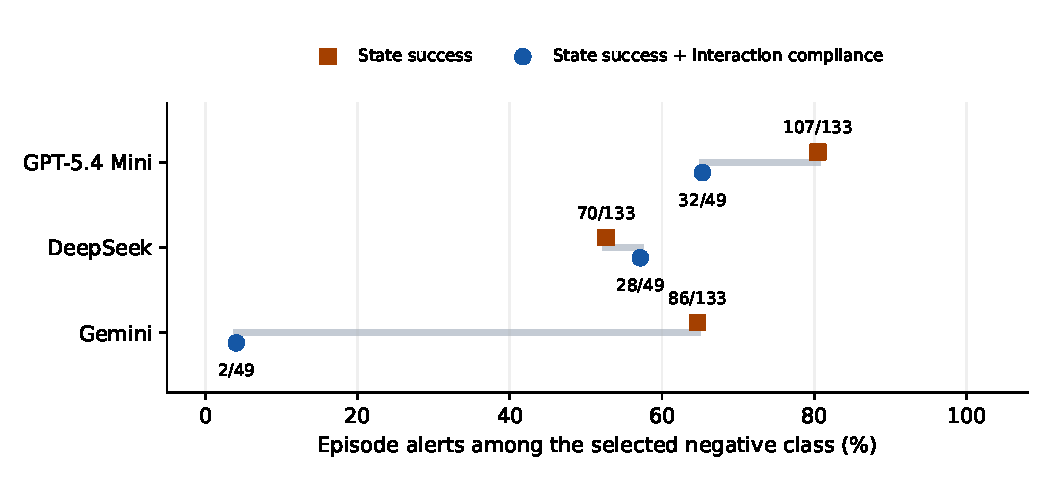
\includegraphics[width=.90\linewidth]{figures/expanded_targets.pdf}
\caption{The same broad-monitor decisions evaluated against two negative classes in the remaining-test expansion. Labels give alert counts and denominators. Gray lines connect the two target-specific rates; colored horizontal spans, where present, show missing-score bounds rather than confidence intervals.}\label{fig:expanded-targets}
\end{figure}
Among 72 task/condition pairs with both repeats completed, 4 change interaction-contract status and 13 change state-success status. These comparisons expose run variability and do not isolate a causal benefit of adding the reminder.

\begin{table}[t]\centering\small
\caption{First-alert timing relative to the first measured interaction violation. Contract-clean conversations are outside this timing denominator.}\label{tab:expanded-timing}
\begin{tabular}{llrrrrr}
\toprule
Cohort & Monitor & Before & At & After & No alert & Unidentified\\
\midrule
Original & Gemini & 0 & 48 & 0 & 0 & 0\\
Original & DeepSeek & 7 & 7 & 14 & 19 & 1\\
Original & GPT-5.4 Mini & 21 & 18 & 5 & 4 & 0\\
Expansion & Gemini & 0 & 103 & 0 & 0 & 0\\
Expansion & DeepSeek & 26 & 11 & 17 & 48 & 1\\
Expansion & GPT-5.4 Mini & 46 & 34 & 12 & 10 & 1\\
\bottomrule
\end{tabular}
\end{table}
\subsection{Constructed substantive-policy contrasts without human labels}
\label{sec:policy-lab}
To test a substantive rule separately from harmless tool batching, we construct 24 matched cancellation pairs: six rule contrasts across four deterministically selected source reservations, with an eligible and an ineligible variant in each pair. The contrasts cover booking age, airline cancellation, business cabin, health insurance, covered weather reason, and a previously flown segment. All prefixes supply the user and reservation IDs, cancellation reason, native reservation and flight-status observations, and explicit confirmation. Each ends with the same single, text-free cancellation proposal within its pair. Labels concern only cancellation eligibility, not comprehensive policy compliance.

Eligibility is computed from explicit simulator facts using two separately written formulations of the stated rule, checked over a factorial grid. This is implementation cross-checking, not independent human adjudication. Boundary-ambiguous exact 24-hour bookings are excluded from the fixtures. All 48 proposed cancellations execute through the native tool, including the 24 ineligible ones; all 48 satisfy the measured interaction contract. This demonstrates a gap between operation execution, interaction formatting, and substantive eligibility within the constructed cases. The operation-executed label is not the native task-success label $G$, and these synthetic probes are not additional autonomous actor conversations.

Each monitor sees the identical public input twice, under the original broad target and a cancellation-eligibility-only target, in alternating order. Ground-truth labels, fixture identifiers, final database state and post-action results are excluded from monitor inputs.
\begin{table}[t]\centering\small
\caption{Constructed policy cases: alerts at threshold 0.5 among 24 eligible and 24 ineligible cancellations. The focused target concerns cancellation eligibility only. Missing scores produce count ranges. These are controlled-case counts, not natural violation prevalence or deployment error estimates.}\label{tab:policy-lab}
\begin{tabular}{llll}
\toprule
Monitor & Target & Eligible alerts & Ineligible alerts\\
\midrule
Gemini & broad & 0/24 & 24/24\\
Gemini & eligibility & 0/24 & 24/24\\
DeepSeek & broad & 0/24 & 16/24\\
DeepSeek & eligibility & 3/24 & 21/24\\
GPT-5.4 Mini & broad & 0/24 & 1/24\\
GPT-5.4 Mini & eligibility & 0/24 & 4/24\\
\bottomrule
\end{tabular}
\end{table}
The artifact reports score-direction changes within every pair and all six rule strata, including failures. Four reused source reservations and six constructed rule contrasts do not form a representative semantic-policy benchmark. No human-labeled accuracy, naturally occurring semantic-violation rate, calibrated risk probability or repair benefit is claimed.
